% =====================================================================
%  Chapter 2 -- Geometry
% =====================================================================
\section{Geometry}

The geometry of the model was built using MCNP~\cite{primer} and inspected with the Visual Editor~\cite{vised}.
An overview of the reactor core is shown in figure~\ref{fig:vised}, where the core is an $8\times9$ lattice of cells, addressed by the column letters $A$ to $H$ and the row numbers $1$ to $9$.
The per cell aluminium casings are not drawn so that the cell contents stay visible, but these are shown later in the cell geometry descriptions.
Each grid position holds a fuel cell, a graphite control cell or a water filled empty cell.

% =====================================================================
%  core.tex  --  full core loaded geometry: the 8x9 lattice of cells, coloured
%  as in the MCNP render.  red = graphite (control cells), yellow = water (empty
%  cells, holes, rod gaps), green = aluminium, blue = UO2 fuel.  Holed control
%  cells show the central aluminium-lined water channel; fuel cells show their
%  4x4 inner lattice grid + rods, with the corner-empty (B3), half-filled (D4)
%  and middle-empty (F3) variants.  Columns A-H (top) and rows 1-9 (left, italic)
%  give the core coordinate system.
%  NB: the cell size is a fixed length (1.81 cm => ~0.95 of the 16 cm text width)
%  rather than a \textwidth fraction.  This is NOT \resizebox -- it only sets the
%  pgf coordinate unit, so fonts and line weights keep their true size.  The rod
%  and grid drawing is inlined (helper macros taking the rod coordinate triggered
%  a spurious "Dimension too large").  \input from chapters/2-geometry.tex.
% =====================================================================
\newcommand{\redcell}[2]{%
  \fill[yellow] (#1-1,9-#2) rectangle (#1,10-#2);
  \fill[red] (#1-0.951,9.049-#2) rectangle (#1-0.049,9.951-#2);
  \draw[thin] (#1-0.951,9.049-#2) rectangle (#1-0.049,9.951-#2);
  \draw (#1-1,9-#2) rectangle (#1,10-#2);}
\newcommand{\yellowcell}[2]{%
  \fill[yellow] (#1-1,9-#2) rectangle (#1,10-#2);
  \draw (#1-1,9-#2) rectangle (#1,10-#2);}
\newcommand{\holedcell}[2]{%
  \fill[yellow] (#1-1,9-#2) rectangle (#1,10-#2);
  \fill[red] (#1-0.951,9.049-#2) rectangle (#1-0.049,9.951-#2);
  \draw[thin] (#1-0.951,9.049-#2) rectangle (#1-0.049,9.951-#2);
  \fill[green!75!black] (#1-0.5,9.5-#2) circle (0.225);
  \draw[thin] (#1-0.5,9.5-#2) circle (0.225);
  \fill[yellow] (#1-0.5,9.5-#2) circle (0.20);
  \draw[thin] (#1-0.5,9.5-#2) circle (0.20);
  \draw (#1-1,9-#2) rectangle (#1,10-#2);}
\newcommand{\fuelbg}[2]{%
  \fill[yellow] (#1-1,9-#2) rectangle (#1,10-#2);
  \draw (#1-1,9-#2) rectangle (#1,10-#2);}
\newcommand{\rodgrid}[2]{%
  \begin{scope}[shift={(#1-0.5,9.5-#2)}]
    \draw[thin] (-0.451,-0.451) rectangle (0.451,0.451);
    \foreach \g in {-0.2257,0,0.2257}{
      \draw[thin] (\g,-0.451) -- (\g,0.451);
      \draw[thin] (-0.451,\g) -- (0.451,\g);}
    \foreach \dx in {-0.3385,-0.1128,0.1128,0.3385}
      \foreach \dy in {-0.3385,-0.1128,0.1128,0.3385}{
        \fill[green!75!black] (\dx,\dy) circle (0.072);
        \draw[thin] (\dx,\dy) circle (0.072);
        \fill[blue] (\dx,\dy) circle (0.046);
        \draw[thin] (\dx,\dy) circle (0.046);}
  \end{scope}}
\begin{figure}[H]
  \centering
  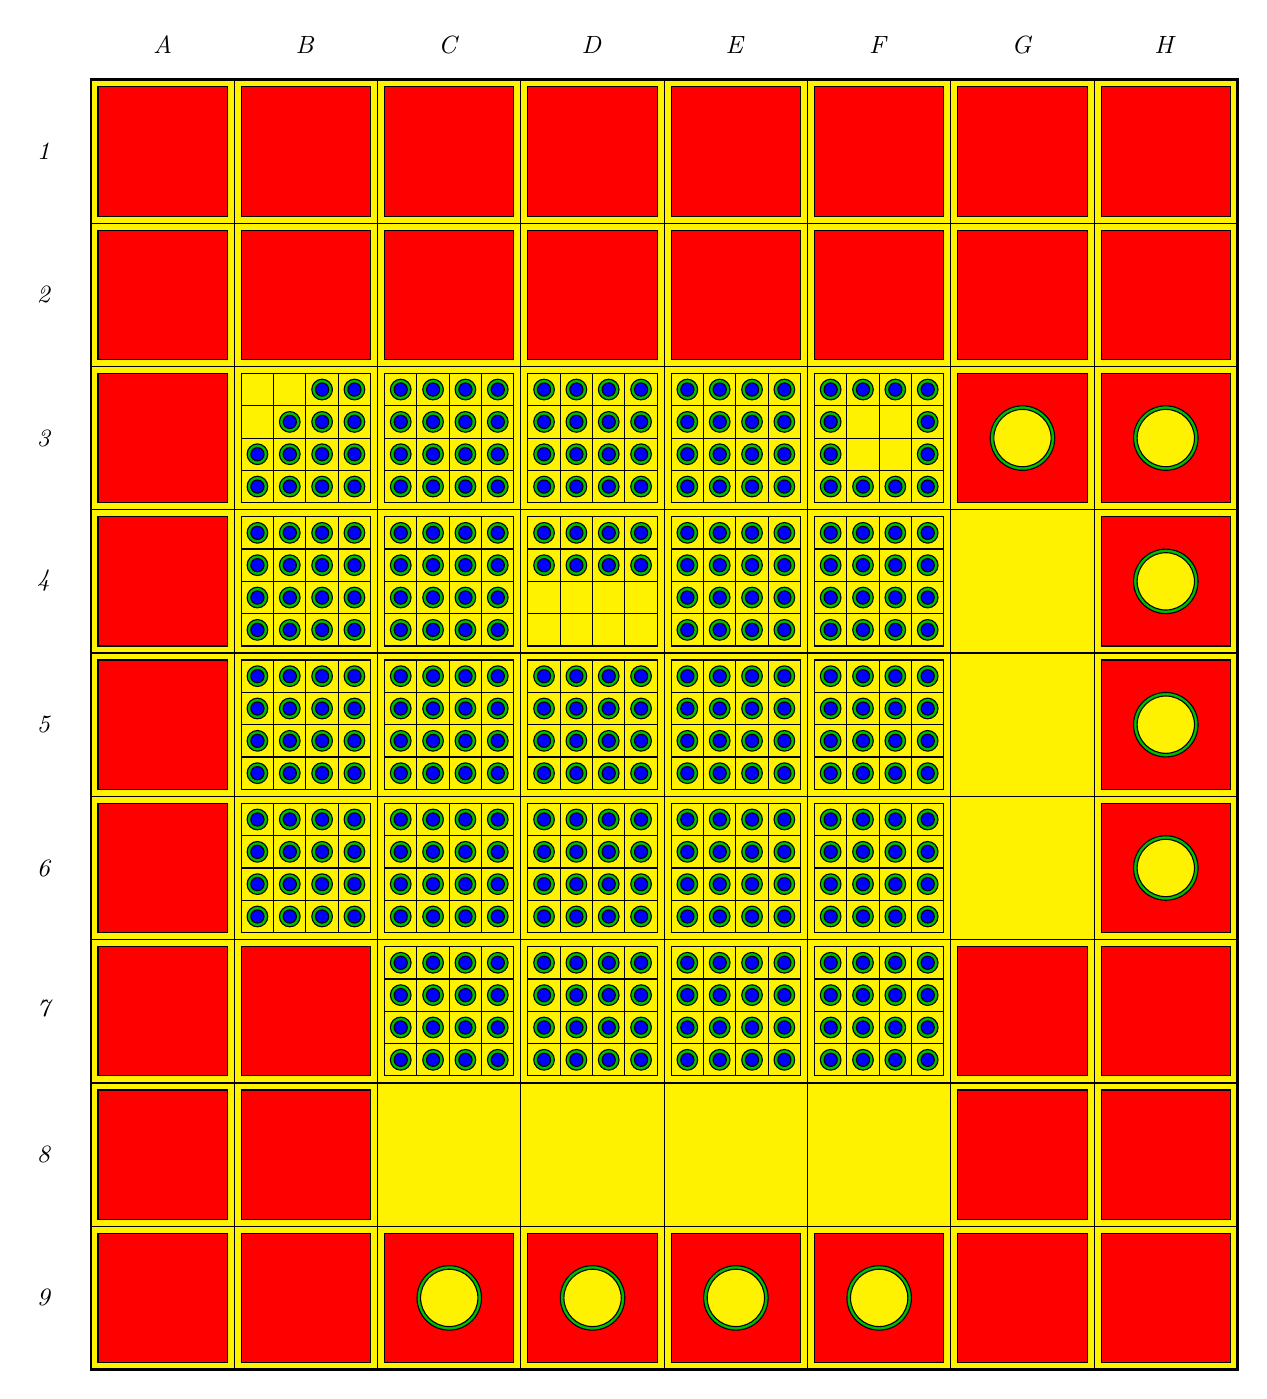
\begin{tikzpicture}[x=1.82cm,y=1.82cm,font=\small]
    \foreach \c/\r in {%
      1/1,2/1,3/1,4/1,5/1,6/1,7/1,8/1,%
      1/2,2/2,3/2,4/2,5/2,6/2,7/2,8/2,%
      1/3,1/4,1/5,1/6,%
      1/7,2/7,7/7,8/7,%
      1/8,2/8,7/8,8/8,%
      1/9,2/9,7/9,8/9}{\redcell{\c}{\r}}
    \foreach \c/\r in {7/4,7/5,7/6,3/8,4/8,5/8,6/8}{\yellowcell{\c}{\r}}
    \foreach \c/\r in {7/3,8/3,8/4,8/5,8/6,3/9,4/9,5/9,6/9}{\holedcell{\c}{\r}}
    \foreach \c/\r in {%
      3/3,4/3,5/3,%
      2/4,3/4,5/4,6/4,%
      2/5,3/5,4/5,5/5,6/5,%
      2/6,3/6,4/6,5/6,6/6,%
      3/7,4/7,5/7,6/7}{\fuelbg{\c}{\r}\rodgrid{\c}{\r}}
    % B3 corner-empty (col 2, row 3): top-left triangle has no rods
    \fuelbg{2}{3}
    \begin{scope}[shift={(1.5,6.5)}]
      \draw[thin] (-0.451,-0.451) rectangle (0.451,0.451);
      \foreach \g in {-0.2257,0,0.2257}{
        \draw[thin] (\g,-0.451) -- (\g,0.451);
        \draw[thin] (-0.451,\g) -- (0.451,\g);}
      \foreach \dx/\dy in {0.1128/0.3385,0.3385/0.3385,%
        -0.1128/0.1128,0.1128/0.1128,0.3385/0.1128,%
        -0.3385/-0.1128,-0.1128/-0.1128,0.1128/-0.1128,0.3385/-0.1128,%
        -0.3385/-0.3385,-0.1128/-0.3385,0.1128/-0.3385,0.3385/-0.3385}{
          \fill[green!75!black] (\dx,\dy) circle (0.072);
          \draw[thin] (\dx,\dy) circle (0.072);
          \fill[blue] (\dx,\dy) circle (0.046);
          \draw[thin] (\dx,\dy) circle (0.046);}
    \end{scope}
    % F3 middle-empty (col 6, row 3): inner 2x2 has no rods
    \fuelbg{6}{3}
    \begin{scope}[shift={(5.5,6.5)}]
      \draw[thin] (-0.451,-0.451) rectangle (0.451,0.451);
      \foreach \g in {-0.2257,0,0.2257}{
        \draw[thin] (\g,-0.451) -- (\g,0.451);
        \draw[thin] (-0.451,\g) -- (0.451,\g);}
      \foreach \dx/\dy in {-0.3385/0.3385,-0.1128/0.3385,0.1128/0.3385,0.3385/0.3385,%
        -0.3385/0.1128,0.3385/0.1128,%
        -0.3385/-0.1128,0.3385/-0.1128,%
        -0.3385/-0.3385,-0.1128/-0.3385,0.1128/-0.3385,0.3385/-0.3385}{
          \fill[green!75!black] (\dx,\dy) circle (0.072);
          \draw[thin] (\dx,\dy) circle (0.072);
          \fill[blue] (\dx,\dy) circle (0.046);
          \draw[thin] (\dx,\dy) circle (0.046);}
    \end{scope}
    % D4 half-filled (col 4, row 4): only the top two rows have rods
    \fuelbg{4}{4}
    \begin{scope}[shift={(3.5,5.5)}]
      \draw[thin] (-0.451,-0.451) rectangle (0.451,0.451);
      \foreach \g in {-0.2257,0,0.2257}{
        \draw[thin] (\g,-0.451) -- (\g,0.451);
        \draw[thin] (-0.451,\g) -- (0.451,\g);}
      \foreach \dx/\dy in {-0.3385/0.3385,-0.1128/0.3385,0.1128/0.3385,0.3385/0.3385,%
        -0.3385/0.1128,-0.1128/0.1128,0.1128/0.1128,0.3385/0.1128}{
          \fill[green!75!black] (\dx,\dy) circle (0.072);
          \draw[thin] (\dx,\dy) circle (0.072);
          \fill[blue] (\dx,\dy) circle (0.046);
          \draw[thin] (\dx,\dy) circle (0.046);}
    \end{scope}
    \draw[line width=1pt] (0,0) rectangle (8,9);
    \foreach \c/\L in {1/A,2/B,3/C,4/D,5/E,6/F,7/G,8/H}
      \node at (\c-0.5,9.24) {\textit{\L}};
    \foreach \r/\L in {1/1,2/2,3/3,4/4,5/5,6/6,7/7,8/8,9/9}
      \node at (-0.32,9.5-\r) {\textit{\L}};
  \end{tikzpicture}
  \caption{Reactor core geometry showing the lattice of cells. The colours represent materials, blue is UO$_2$ fuel, green is aluminum, yellow is water and red is graphite.}
  \label{fig:vised}
\end{figure}


\newpage

\subsection{Fuel Rod}

The fuel rod is modelled as two coaxial cylinders, a UO$_2$ fuel meat enclosed in an aluminium cladding.
Its principal dimensions are given in the blueprint of figure~\ref{fig:fuelrod}.

% =====================================================================
%  fuel_rod.tex  --  blueprint of the fuel rod.  Front view (left) shows the
%  two lengths (cladding 590, fuel meat 500); left view (right) shows the two
%  concentric diameters (cladding 10, fuel meat 7).  Dash-dot symmetry centre-
%  lines.  Lengths foreshortened (not to scale); dimensions in mm.
%  \input from chapters/2-geometry.tex.
% =====================================================================
\begin{figure}[H]
  \centering
  \begin{tikzpicture}[
      font=\small,
      dim/.style ={{Stealth[length=1.6mm]}-{Stealth[length=1.6mm]}, thin},
      ext/.style ={thin},
      lead/.style={-{Stealth[length=1.4mm]}, thin},
      cl/.style  ={thin, dash pattern=on 7pt off 2pt on 1pt off 2pt},
      almat/.style  ={pattern={Lines[angle=60,distance=3pt,line width=0.4pt]},
                      pattern color=green!75!black},
      fuelmat/.style={pattern=crosshatch, pattern color=blue},
    ]
    % ---- material hatching: Al cladding (green 60-deg lines), UO2 fuel meat
    %      (blue cross-hatch).  Lay down green, erase the fuel area with white,
    %      then cross-hatch it, so the two patterns never overlap. ------------
    % front view (left), as a longitudinal section
    \fill[almat]   (0,-0.7) rectangle (8,0.7);
    \fill[white]   (0.61,-0.49) rectangle (7.39,0.49);
    \fill[fuelmat] (0.61,-0.49) rectangle (7.39,0.49);
    % left view (right), cross-section
    \fill[almat]   (10.5,0) circle (0.70);
    \fill[white]   (10.5,0) circle (0.49);
    \fill[fuelmat] (10.5,0) circle (0.49);

    % ---- outlines ---------------------------------------------------------
    \draw[thick] (0,-0.7) rectangle (8,0.7);            % Al cladding, L = 590
    \draw[thick] (0.61,-0.49) rectangle (7.39,0.49);    % UO2 fuel meat, l = 500
    \draw[thick] (10.5,0) circle (0.70);                % Al cladding, D = 10
    \draw[thick] (10.5,0) circle (0.49);                % UO2 fuel meat, D = 7

    % ---- symmetry centrelines (dash-dot) ----------------------------------
    \draw[cl] (-0.6,0) -- (11.9,0);                     % common horizontal axis
    \draw[cl] (4,-0.95) -- (4,0.95);                    % front view, mid-length
    \draw[cl] (10.5,-0.95) -- (10.5,0.95);              % left view, vertical

    % ---- length dimensions (front view) -----------------------------------
    \draw[ext] (0.61,-0.59) -- (0.61,-1.58);            % l = 500 (inner fuel)
    \draw[ext] (7.39,-0.59) -- (7.39,-1.58);
    \draw[dim] (0.61,-1.45) -- (7.39,-1.45);
    \node[fill=white,inner sep=1.5pt] at (4,-1.45) {500};
    \draw[ext] (0,-0.8) -- (0,-2.03);                   % L = 590 (cladding)
    \draw[ext] (8,-0.8) -- (8,-2.03);
    \draw[dim] (0,-1.9) -- (8,-1.9);
    \node[fill=white,inner sep=1.5pt] at (4,-1.9) {590};

    % ---- diameter dimensions (left view) ----------------------------------
    \draw[lead] (11.9,0.95) -- (11.6,0.95) -- (10.90,0.573);   % D = 10 (outer)
    \node[anchor=west] at (11.95,0.95) {\O 10};
    \draw[lead] (9.3,-0.85) -- (9.6,-0.85) -- (10.22,-0.40);   % D = 7 (inner)
    \node[anchor=east] at (9.25,-0.85) {\O 7};
  \end{tikzpicture}
  \caption{Dimensions of a fuel rod in mm.}
  \label{fig:fuelrod}
\end{figure}


\subsection{Cells}

The fuel rods are fitted into a $4\times4$ lattice inside an aluminium casing, which together form a fuel cell.
Its top view dimensions are shown in figure~\ref{fig:fuelcell}.

% =====================================================================
%  fuel_cell.tex  --  top view of a fuel cell, coloured as in the MCNP render
%  (yellow water, green aluminium, blue UO2).  A 4x4 fuel-rod lattice sits in an
%  aluminium box.  Dimensions: lattice element b = 1.625 and cell pitch e = 7.2
%  (bottom), Al box side a = 6.5 (right); all cm.  The italic indices on the top
%  (columns, i) and left (rows, j) are the MCNP lattice coordinates
%  (fill=-1:2 -1:2), so a rod is addressed as i:j.
%  \input from chapters/2-geometry.tex.
% =====================================================================
\begin{figure}[H]
  \centering
  \begin{tikzpicture}[
      scale=0.8,
      font=\small,
      dim/.style ={{Stealth[length=1.6mm]}-{Stealth[length=1.6mm]}, thin},
      ext/.style ={thin},
    ]
    % phantom points: balance the bounding box about the cell centre (x=0) so the
    % square stays centred in the figure despite the right-side dimensions
    % (real content spans x in [-4.35, 5.33]; +-5.4 brackets it symmetrically).
    \path (-5.4,0) (5.4,0);
    % ---- materials (coloured like the MCNP top view) ----
    \fill[yellow]          (-3.6,-3.6)   rectangle (3.6,3.6);    % water (cell)
    \fill[green!75!black]  (-3.4,-3.4)   rectangle (3.4,3.4);    % Al box wall
    \fill[yellow]          (-3.25,-3.25) rectangle (3.25,3.25);  % water cavity (a)
    % 4x4 lattice grid lines
    \foreach \i in {-1.625,0,1.625}{
      \draw[thin] (\i,-3.25) -- (\i,3.25);
      \draw[thin] (-3.25,\i) -- (3.25,\i);
    }
    % fuel rods: Al cladding (green) + UO2 meat (blue)
    \foreach \x in {-2.4375,-0.8125,0.8125,2.4375}{
      \foreach \y in {-2.4375,-0.8125,0.8125,2.4375}{
        \fill[green!75!black] (\x,\y) circle (0.5);
        \fill[blue]           (\x,\y) circle (0.35);
        \draw[thin]           (\x,\y) circle (0.5);
        \draw[thin]           (\x,\y) circle (0.35);
      }
    }
    % ---- outlines ----
    \draw[thick] (-3.6,-3.6)   rectangle (3.6,3.6);     % cell pitch (e)
    \draw        (-3.4,-3.4)   rectangle (3.4,3.4);     % Al box outer wall
    \draw        (-3.25,-3.25) rectangle (3.25,3.25);   % Al box cavity (a)

    % ---- lattice coordinates (MCNP fill=-1:2 -1:2): columns i on top, rows j on left ----
    \foreach \x/\lab in {-2.4375/-1,-0.8125/0,0.8125/1,2.4375/2}
      \node at (\x,3.95) {\textit{\lab}};
    \foreach \y/\lab in {2.4375/-1,0.8125/0,-0.8125/1,-2.4375/2}
      \node at (-4.15,\y) {\textit{\lab}};

    % ---- dimensions ----
    % b = 1.625 (one lattice element) -- bottom, just under the square
    \draw[ext] (-3.25,-3.35)  -- (-3.25,-4.1);
    \draw[ext] (-1.625,-3.35) -- (-1.625,-4.1);
    \draw[dim] (-3.25,-4.0)   -- (-1.625,-4.0);
    \node[fill=white,inner sep=1.5pt] at (-2.4375,-4.0) {1.625};
    % e = 7.2 (whole cell side) -- bottom, below the 1.625
    \draw[ext] (-3.6,-3.7) -- (-3.6,-4.85);
    \draw[ext] (3.6,-3.7)  -- (3.6,-4.85);
    \draw[dim] (-3.6,-4.7) -- (3.6,-4.7);
    \node[fill=white,inner sep=1.5pt] at (0,-4.7) {7.2};
    % a = 6.5 (Al box cavity side) -- right, inner
    \draw[ext] (3.35,3.25)  -- (4.5,3.25);
    \draw[ext] (3.35,-3.25) -- (4.5,-3.25);
    \draw[dim] (4.35,-3.25) -- (4.35,3.25);
    \node[fill=white,inner sep=1.5pt,rotate=90] at (4.35,0) {6.5};
    % 6.8 = Al casing outer side -- right, outside the 6.5
    \draw[ext] (3.5,3.4)   -- (5.3,3.4);
    \draw[ext] (3.5,-3.4)  -- (5.3,-3.4);
    \draw[dim] (5.15,-3.4) -- (5.15,3.4);
    \node[fill=white,inner sep=1.5pt,rotate=90] at (5.15,0) {6.8};
  \end{tikzpicture}
  \caption{Top view of a fuel cell. A rod is adressed with the lattice coordinates, columns $i$ and rows $j$. The dimensions are in cm.}
  \label{fig:fuelcell}
\end{figure}


The height of each cell, and therefore the whole reactor core is $60~\mathrm{cm}$.

\newpage

Besides the fully loaded cell, three partially loaded fuel cell variants occur in the core, a half-filled, a middle-empty and a corner-empty arrangement, shown in figure~\ref{fig:fuelcelltypes}.
In each variant the omitted lattice positions are left as water.

% =====================================================================
%  fuel_cell_types.tex  --  the three partially loaded fuel-cell variants that
%  occur in the core, drawn like the fuel-cell square of Figure~\ref{fig:fuelcell}
%  but with no dimensions or labels.  Left: half-filled (only the top two rod rows
%  loaded); middle: middle-empty (inner 2x2 unloaded); right: corner-empty (the
%  top-left corner triangle unloaded).  The omitted lattice positions stay water
%  (yellow).  Three cells side by side; the coordinate unit (0.524 cm = 80%% of
%  the earlier 0.655 cm) sets the total width to ~0.76 of the 16 cm text width --
%  NOT \resizebox.
%  \input from chapters/2-geometry.tex.
% =====================================================================
\newcommand{\fctypebase}{%
  \fill[yellow]          (-3.6,-3.6)   rectangle (3.6,3.6);    % water (cell)
  \fill[green!75!black]  (-3.4,-3.4)   rectangle (3.4,3.4);    % Al box wall
  \fill[yellow]          (-3.25,-3.25) rectangle (3.25,3.25);  % water cavity
  \foreach \g in {-1.625,0,1.625}{
    \draw[thin] (\g,-3.25) -- (\g,3.25);
    \draw[thin] (-3.25,\g) -- (3.25,\g);}
  \draw[thick] (-3.6,-3.6)   rectangle (3.6,3.6);
  \draw        (-3.4,-3.4)   rectangle (3.4,3.4);
  \draw        (-3.25,-3.25) rectangle (3.25,3.25);}
\begin{figure}[H]
  \centering
  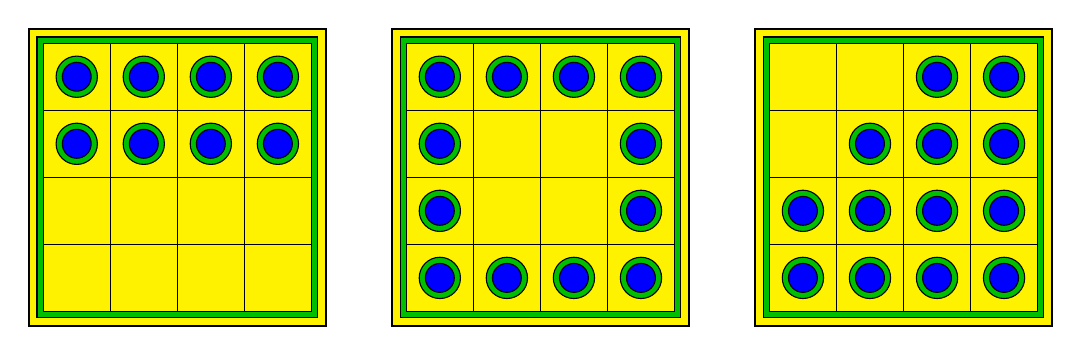
\begin{tikzpicture}[x=0.524cm,y=0.524cm]
    % ---- left: half-filled (top two rod rows only) ----
    \begin{scope}[shift={(0,0)}]
      \fctypebase
      \foreach \x/\y in {%
        -2.4375/2.4375,-0.8125/2.4375,0.8125/2.4375,2.4375/2.4375,%
        -2.4375/0.8125,-0.8125/0.8125,0.8125/0.8125,2.4375/0.8125}{
          \fill[green!75!black] (\x,\y) circle (0.5);
          \draw[thin]           (\x,\y) circle (0.5);
          \fill[blue]           (\x,\y) circle (0.35);
          \draw[thin]           (\x,\y) circle (0.35);}
    \end{scope}
    % ---- middle: middle-empty (inner 2x2 unloaded) ----
    \begin{scope}[shift={(8.8,0)}]
      \fctypebase
      \foreach \x/\y in {%
        -2.4375/2.4375,-0.8125/2.4375,0.8125/2.4375,2.4375/2.4375,%
        -2.4375/0.8125,2.4375/0.8125,%
        -2.4375/-0.8125,2.4375/-0.8125,%
        -2.4375/-2.4375,-0.8125/-2.4375,0.8125/-2.4375,2.4375/-2.4375}{
          \fill[green!75!black] (\x,\y) circle (0.5);
          \draw[thin]           (\x,\y) circle (0.5);
          \fill[blue]           (\x,\y) circle (0.35);
          \draw[thin]           (\x,\y) circle (0.35);}
    \end{scope}
    % ---- right: corner-empty (top-left corner triangle unloaded) ----
    \begin{scope}[shift={(17.6,0)}]
      \fctypebase
      \foreach \x/\y in {%
        0.8125/2.4375,2.4375/2.4375,%
        -0.8125/0.8125,0.8125/0.8125,2.4375/0.8125,%
        -2.4375/-0.8125,-0.8125/-0.8125,0.8125/-0.8125,2.4375/-0.8125,%
        -2.4375/-2.4375,-0.8125/-2.4375,0.8125/-2.4375,2.4375/-2.4375}{
          \fill[green!75!black] (\x,\y) circle (0.5);
          \draw[thin]           (\x,\y) circle (0.5);
          \fill[blue]           (\x,\y) circle (0.35);
          \draw[thin]           (\x,\y) circle (0.35);}
    \end{scope}
  \end{tikzpicture}
  \caption{The three partially loaded fuel-cell variants.}
  \label{fig:fuelcelltypes}
\end{figure}


The control cells use the same outer aluminium casing but are filled with graphite instead of fuel rods.
Some are fully filled, while the holed control cells contain a central, aluminium-lined water channel.
Both types are shown in figure~\ref{fig:controlcell}.

% =====================================================================
%  control_cell.tex  --  top view of the two control-cell types, coloured as in
%  the MCNP render (yellow water, green aluminium, red graphite).  Left: a fully
%  graphite-filled control cell (no hole).  Right: a holed control cell, where a
%  central water hole (bore d = 2.9) is lined by an aluminium wall (w = 1.5 mm),
%  giving an outer diameter of 3.2; only this hole is dimensioned (all cm).  Both
%  diameters are placed on the right of the holed cell (outer high, inner low) so
%  they clear the filled cell on the left.  The cells use the same coordinate unit
%  (0.524 cm) as fuel_cell_types.tex, so the squares are the same size.
%  \input from chapters/2-geometry.tex.
% =====================================================================
\begin{figure}[H]
  \centering
  \begin{tikzpicture}[
      x=0.524cm,y=0.524cm,
      font=\small,
      lead/.style={-{Stealth[length=1.4mm]}, thin},
    ]
    % phantom points: balance the bounding box about the pair midpoint (x=4.4) so
    % the two cells stay centred despite the holed cell's right-side dimensions.
    \path (-5.5,0) (14.3,0);
    % ===== left: fully filled graphite control cell (no hole) =====
    \begin{scope}[shift={(0,0)}]
      \fill[yellow]         (-3.6,-3.6)   rectangle (3.6,3.6);    % water (cell)
      \fill[green!75!black] (-3.4,-3.4)   rectangle (3.4,3.4);    % Al box wall
      \fill[red]            (-3.25,-3.25) rectangle (3.25,3.25);  % graphite (cavity)
      \draw[thick] (-3.6,-3.6)   rectangle (3.6,3.6);     % cell pitch
      \draw        (-3.4,-3.4)   rectangle (3.4,3.4);     % Al box outer wall
      \draw        (-3.25,-3.25) rectangle (3.25,3.25);   % Al box cavity
    \end{scope}
    % ===== right: holed control cell (dimensioned) =====
    \begin{scope}[shift={(8.8,0)}]
      \fill[yellow]         (-3.6,-3.6)   rectangle (3.6,3.6);    % water (cell)
      \fill[green!75!black] (-3.4,-3.4)   rectangle (3.4,3.4);    % Al box wall
      \fill[red]            (-3.25,-3.25) rectangle (3.25,3.25);  % graphite (cavity)
      \fill[green!75!black] (0,0) circle (1.6);                   % Al wall (D = 3.2)
      \fill[yellow]         (0,0) circle (1.45);                  % water hole (D = 2.9)
      \draw[thick] (-3.6,-3.6)   rectangle (3.6,3.6);     % cell pitch
      \draw        (-3.4,-3.4)   rectangle (3.4,3.4);     % Al box outer wall
      \draw        (-3.25,-3.25) rectangle (3.25,3.25);   % Al box cavity
      \draw        (0,0) circle (1.6);
      \draw        (0,0) circle (1.45);
      % ---- diameter dimensions on the right: outer (D 3.2) high, inner (D 2.9) low ----
      \draw[lead] (3.9,1.8)  -- (1.453,0.671);            % D = 3.2 (Al wall, outer)
      \node[anchor=west,fill=white,inner sep=1.5pt] at (3.95,1.8) {\O 3.2};
      \draw[lead] (3.9,-1.8) -- (1.317,-0.608);           % D = 2.9 (water bore, inner)
      \node[anchor=west,fill=white,inner sep=1.5pt] at (3.95,-1.8) {\O 2.9};
    \end{scope}
  \end{tikzpicture}
  \caption{Top view of the two control-cell types.}
  \label{fig:controlcell}
\end{figure}


In the MCNP input file each cell type is a separate universe, empty cells in the reactor core are filled with water.

\newpage

\subsection{Container \& Importance Layers}

The whole core is submerged in water, which has a diameter of 140 cm, and a cylindrical concrete container surrounds that, the width of the container wall is 50 cm and the height is 200 cm.
Both cylinders are divided into 10 cm wide concentric importance layers, with the neutron importance doubled from one shell to the next.
Their top view layout is shown in figure~\ref{fig:implayers}.

% =====================================================================
%  importance_layers.tex  --  top view of the concentric cylindrical importance
%  layers around the core (MCNP cells 200-208, surfaces 61-68).  TWO diagrams:
%  (top)    coloured by material -- water (yellow, r 0-70), concrete (magenta,
%           70-120) -- only the water/concrete mantles (r=70, r=120) are labelled;
%  (bottom) the SAME geometry coloured by a heat map of the neutron importance
%           (imp:n = 1 in the core, then 2,4,...,256 outward).  The importance
%           values (\texttt) are called out on the RIGHT with arrows pointing to
%           the middle of each layer; the diameters are repeated on the LEFT.
%  Core = red / imp=1 rectangle (true 8:9 ratio).  scale=0.02778 -> each diagram
%  is 7 cm tall; phantom points keep the circles centred (NOT \resizebox).
%  \input from chapters/2-geometry.tex.
% =====================================================================
\definecolor{imp1}{HTML}{1F2AFF}
\definecolor{imp2}{HTML}{2A8CFF}
\definecolor{imp4}{HTML}{24D6D6}
\definecolor{imp8}{HTML}{2BD98A}
\definecolor{imp16}{HTML}{6DDB2B}
\definecolor{imp32}{HTML}{C3DB2B}
\definecolor{imp64}{HTML}{FFD42B}
\definecolor{imp128}{HTML}{FF8C2B}
\definecolor{imp256}{HTML}{FF2A2A}
\begin{figure}[H]
  \centering
  % ===== TOP: coloured by material =====
  \begin{tikzpicture}[
      scale=0.02778,   % 252 units (centreline span, +-126) x 0.02778 = 7 cm tall
      font=\small,
      lead/.style={-{Stealth[length=1.6mm]}, thin},
      cl/.style  ={thin, dash pattern=on 7pt off 2pt on 1pt off 2pt},
    ]
    \fill[magenta] (0,0) circle (120);
    \fill[yellow]  (0,0) circle (70);
    \fill[red]   (-28.8,-32.4) rectangle (28.8,32.4);
    \draw[thick] (-28.8,-32.4) rectangle (28.8,32.4);
    % only the water/concrete mantles (importance-layer circles removed)
    \draw[thin] (0,0) circle (70);
    \draw[thin] (0,0) circle (120);
    \draw[cl] (-126,0) -- (126,0);
    \draw[cl] (0,-126) -- (0,126);
    % mantle + core labels with radial leaders (as in the lower diagram)
    \node[anchor=east, align=center, fill=white, inner sep=2pt] (om) at (-152,-60)
      {concrete\\outer\\mantle};
    \draw[lead] (om.east) -- (-111.6,-44.1);          % radial to r=120
    \node[anchor=west, align=center, fill=white, inner sep=2pt] (im) at (152,60)
      {concrete\\inner\\mantle};
    \draw[lead] (im.west) -- (65.1,25.7);             % radial to r=70
    \node[anchor=west, align=center, fill=white, inner sep=2pt] (rc) at (152,-60)
      {reactor\\core};
    \draw[lead] (rc.west) -- (18.6,-7.3);             % radial into the core
    \path (-212,0) (212,0);
  \end{tikzpicture}\\[5mm]
  % ===== BOTTOM: coloured by a heat map of the neutron importance =====
  \begin{tikzpicture}[
      scale=0.02778,
      font=\small,
      lead/.style={-{Stealth[length=1.6mm]}, thin},
      cl/.style  ={thin, dash pattern=on 7pt off 2pt on 1pt off 2pt},
    ]
    % importance heat map (outer shell = highest importance)
    \foreach \r/\c in {120/imp256,110/imp128,100/imp64,90/imp32,80/imp16,70/imp8,60/imp4,50/imp2}
      \fill[\c] (0,0) circle (\r);
    \fill[imp1]  (-28.8,-32.4) rectangle (28.8,32.4);
    \draw[thick] (-28.8,-32.4) rectangle (28.8,32.4);
    \foreach \r in {50,60,70,80,90,100,110,120}
      \draw[thin] (0,0) circle (\r);
    \draw[cl] (-126,0) -- (126,0);
    \draw[cl] (0,-126) -- (0,126);
    % left: diameter callouts to the circles (as in the top diagram)
    \foreach \d/\tx/\ty/\ly in {%
        240/-98.3/68.8/105, 220/-98.4/49.2/75, 200/-95.8/28.7/45, 180/-89.6/9.0/15,%
        160/-79.6/-8.0/-15, 140/-67.0/-20.1/-45, 120/-53.7/-26.8/-75, 100/-41.0/-28.7/-105}{
      \draw[lead] (-150,\ly) -- (\tx,\ty);
      \node[anchor=east,fill=white,inner sep=1pt] at (-150,\ly) {\O \d};
    }
    % right: importance callouts (monospace), arrows to the middle of each layer
    \foreach \v/\tx/\ty/\ly in {%
        256/92.1/68.8/112, 128/91.6/51.3/84, 64/89.0/33.2/56, 32/83.6/15.6/28,%
        16/75.0/0/0, 8/63.9/-11.9/-28, 4/51.5/-19.2/-56, 2/36.7/-20.5/-84,%
        1/14.4/-10.8/-112}{
      \draw[lead] (150,\ly) -- (\tx,\ty);
      \node[anchor=west,fill=white,inner sep=1pt] at (150,\ly) {\texttt{imp:n=\v}};
    }
    \path (-222,0) (222,0);
  \end{tikzpicture}
  \caption{Importance layers around the core, coloured by material
    (top) and by neutron importance (bottom). The diameters are in cm.}
  \label{fig:implayers}
\end{figure}


The diameter of the innermost layer is set so that it fully encloses the reactor core.
The effective diameter of the core is the diagonal of the $8\times9$ lattice with a cell pitch of $p=7.2~\mathrm{cm}$, given by the following equation.

\begin{equation}
D_\mathrm{core} = \sqrt{(8p)^2 + (9p)^2} = p\sqrt{8^2 + 9^2} = 7.2\sqrt{145}~\mathrm{cm} \approx 86.7~\mathrm{cm}.
\end{equation}

The innermost layer is given a diameter of $100~\mathrm{cm}$, the smallest round value that still contains the whole core.

\newpage
